\begin{figure}[htbp]\centering
\begin{subfigure}[t]{0.32\linewidth}\centering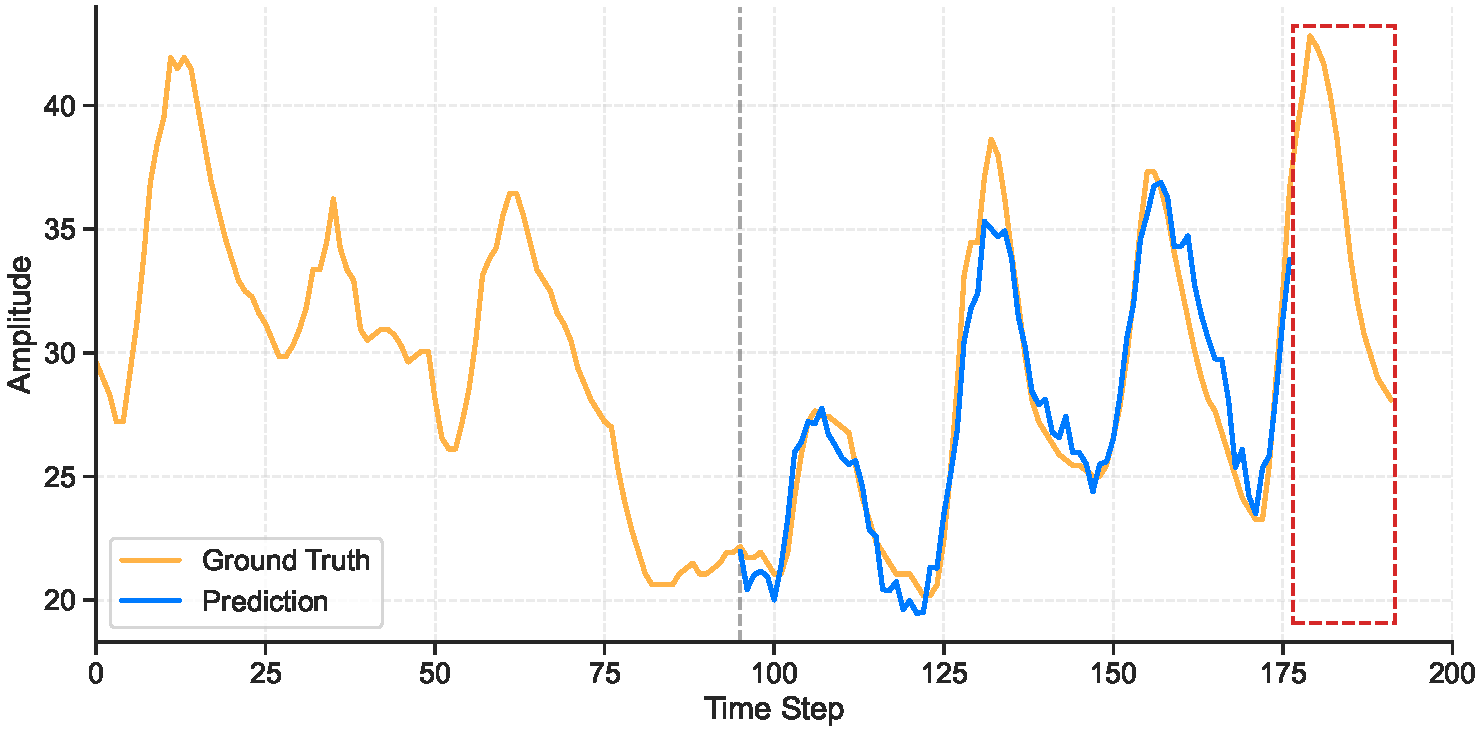
\includegraphics[width=\linewidth]{figures/appendix/showcase_additional/ground_truth_plot_01_len.pdf}\caption{Incomplete prediction (early stopping).}\label{fig:showcase01_add01-len}\end{subfigure}%
\hfill%
\begin{subfigure}[t]{0.32\linewidth}\centering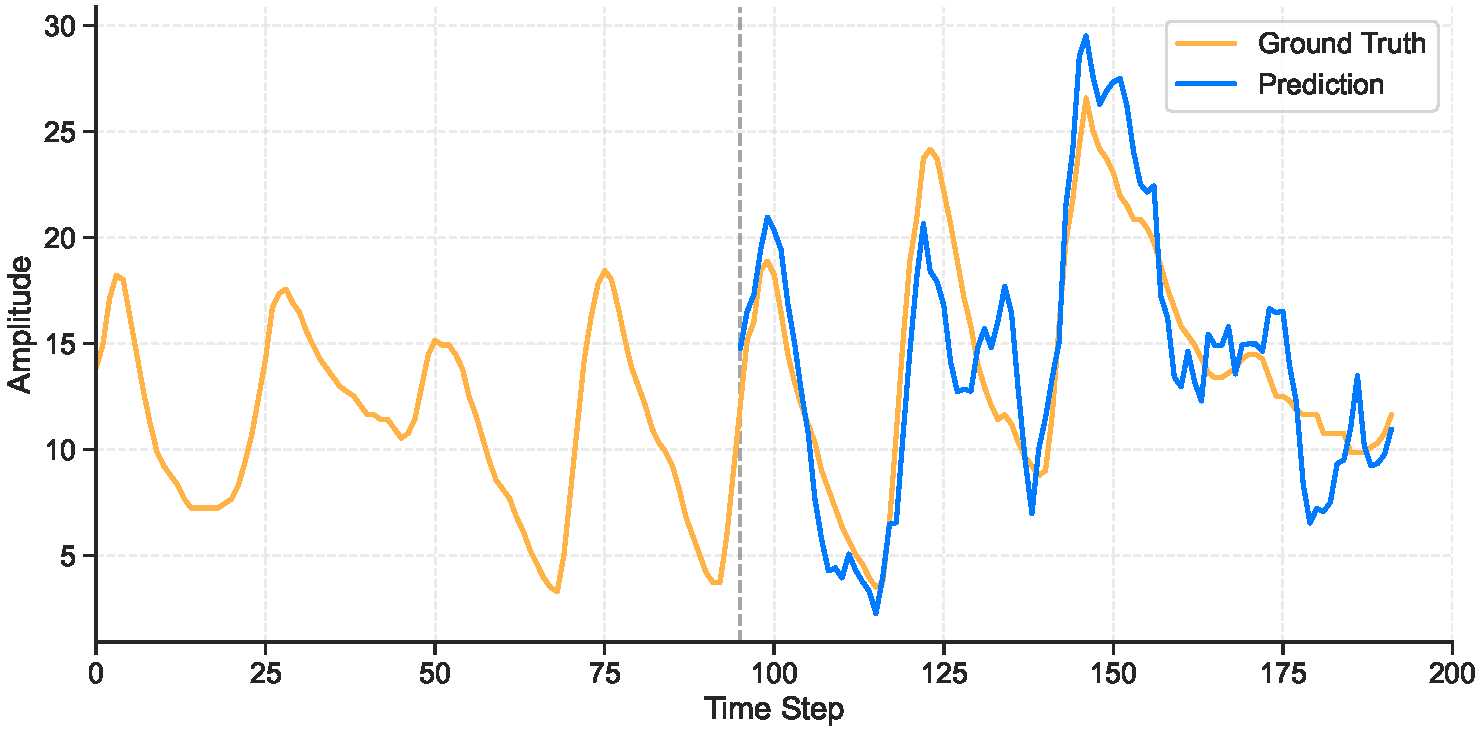
\includegraphics[width=\linewidth]{figures/appendix/showcase_additional/ground_truth_plot_02_mse.pdf}\caption{Low prediction accuracy (high MSE).}\label{fig:showcase02_add01-mse}\end{subfigure}%
\hfill%
\begin{subfigure}[t]{0.32\linewidth}\centering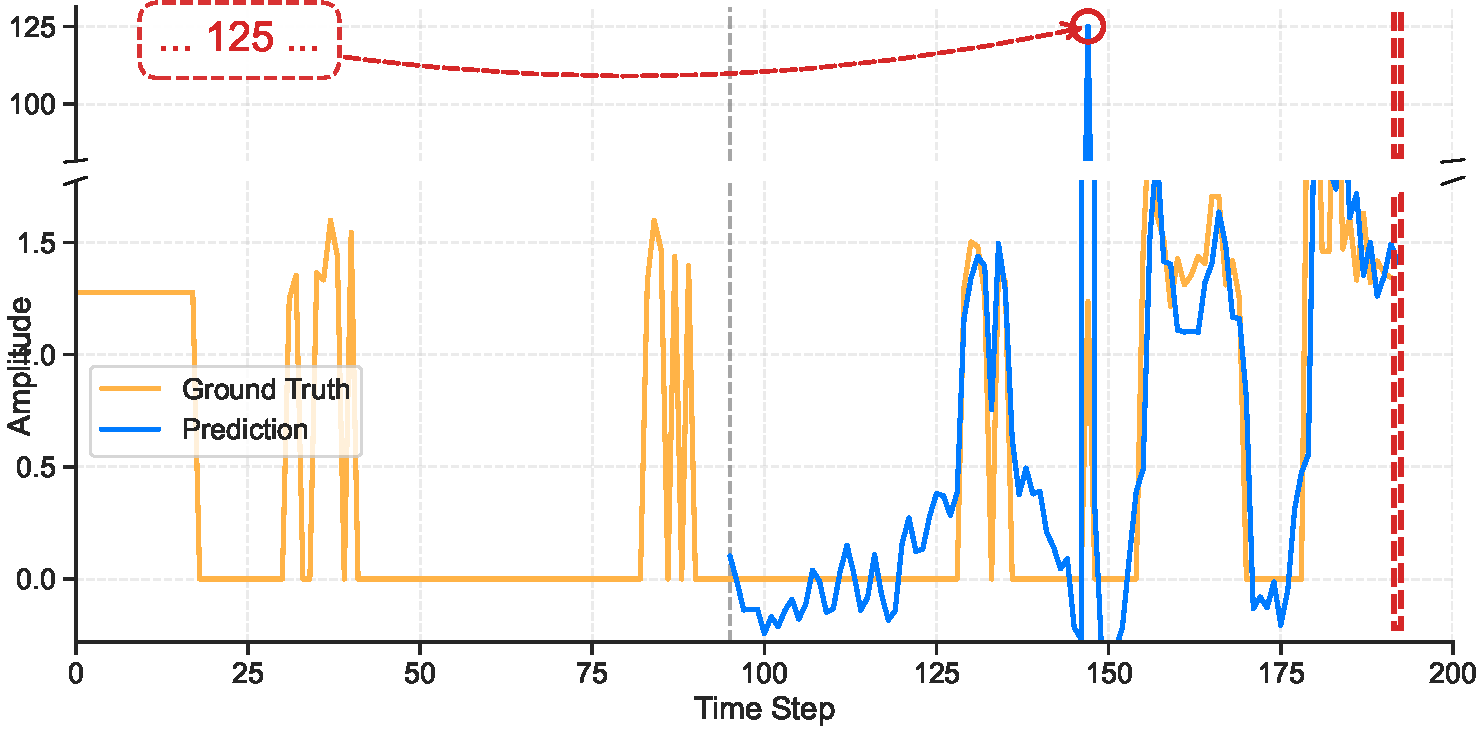
\includegraphics[width=\linewidth]{figures/appendix/showcase_additional/ground_truth_plot_03_decimal.pdf}\caption{Formatting error causing abnormal spikes.}\label{fig:showcase03_add01-fmt}\end{subfigure}%
\par\medskip
\begin{subfigure}[t]{0.32\linewidth}\centering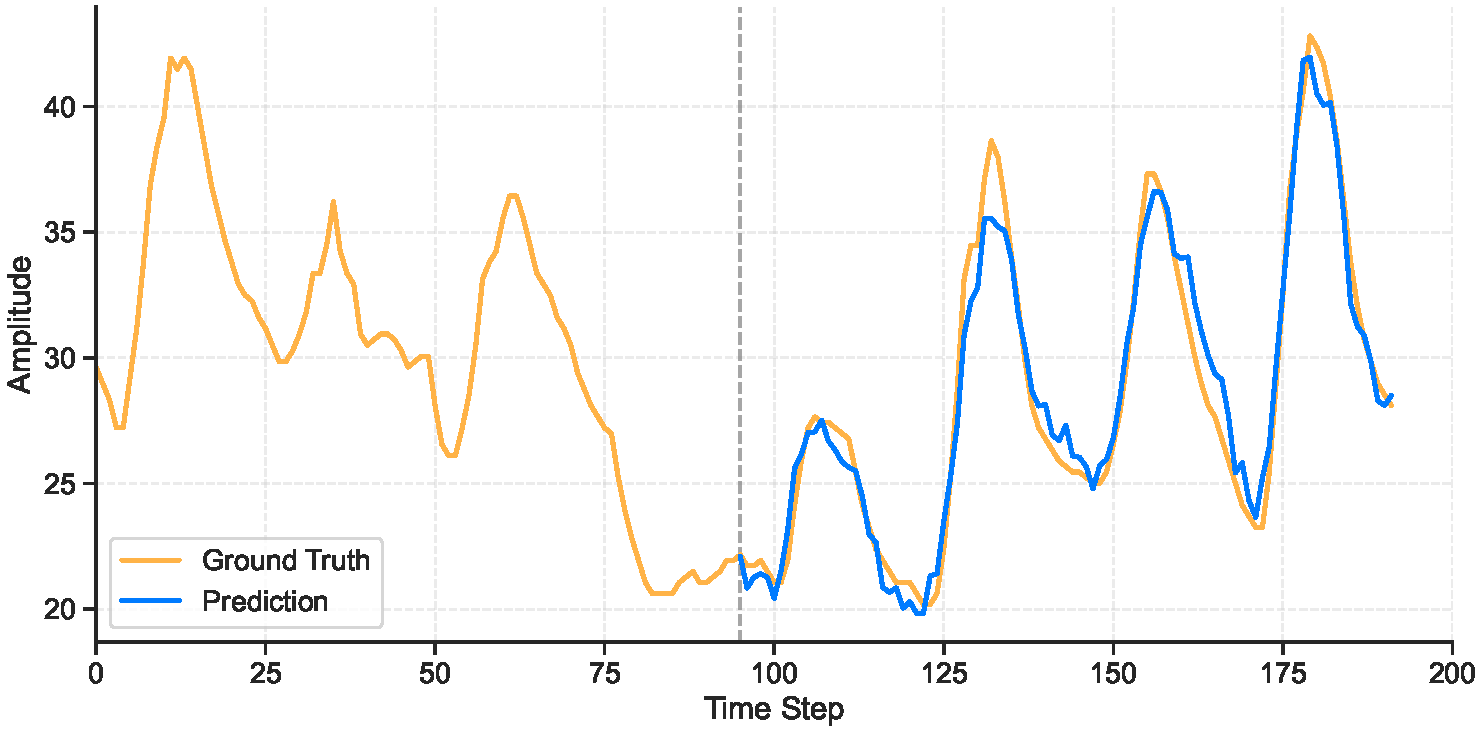
\includegraphics[width=\linewidth]{figures/appendix/showcase_additional/ground_truth_plot_01.pdf}\caption{Correction of prediction length.}\label{fig:showcase01_add01}\end{subfigure}%
\hfill%
\begin{subfigure}[t]{0.32\linewidth}\centering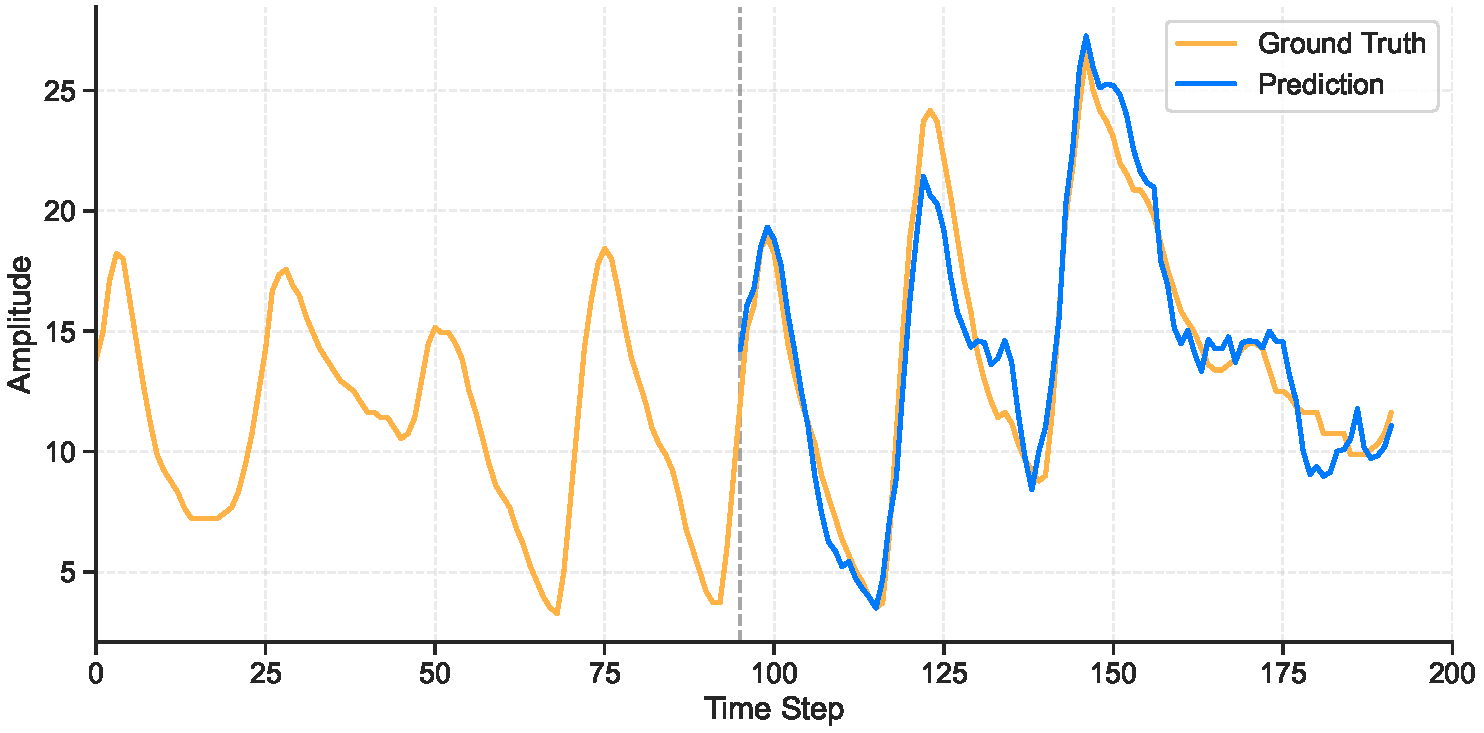
\includegraphics[width=\linewidth]{figures/appendix/showcase_additional/ground_truth_plot_02.pdf}\caption{Enhanced prediction precision.}\label{fig:showcase02_add01}\end{subfigure}%
\hfill%
\begin{subfigure}[t]{0.32\linewidth}\centering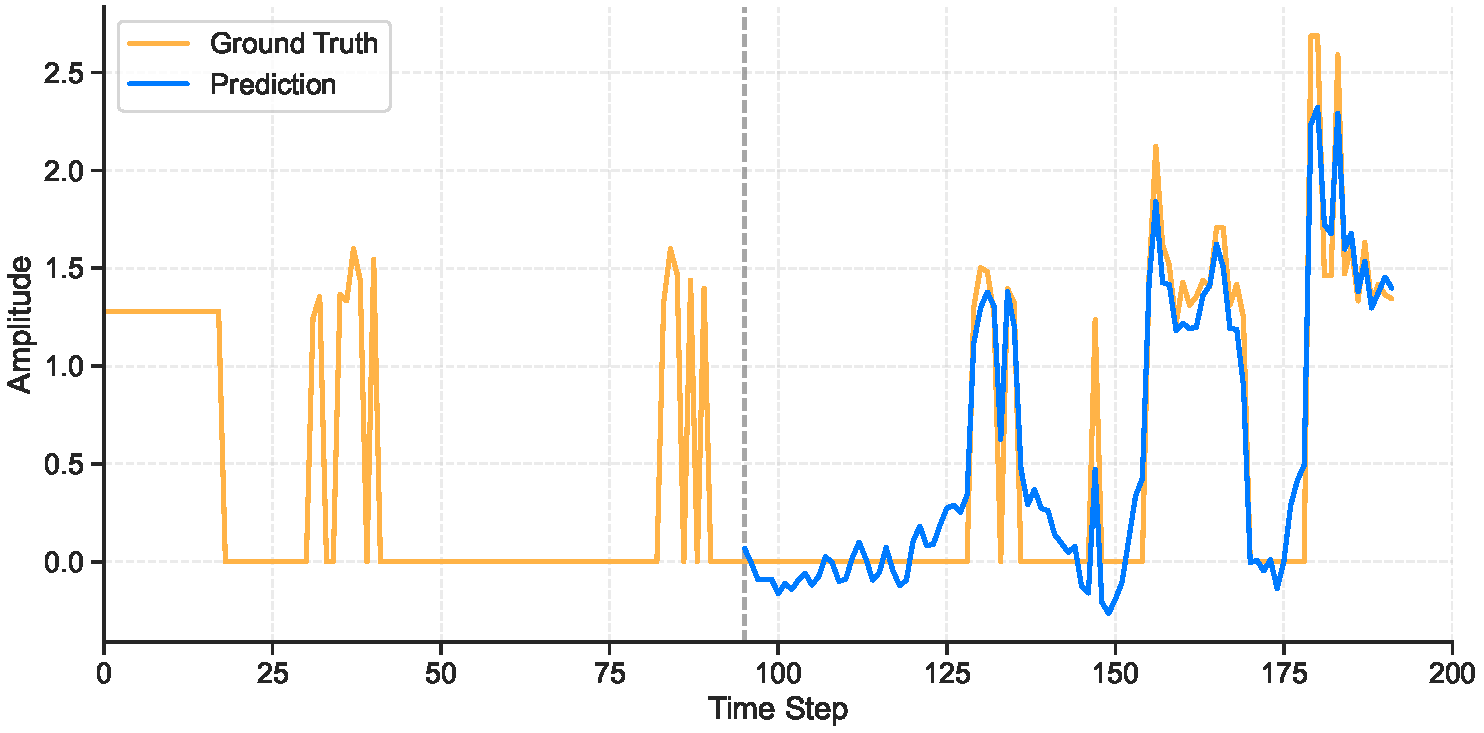
\includegraphics[width=\linewidth]{figures/appendix/showcase_additional/ground_truth_plot_03.pdf}\caption{Rectification of output format and outliers.}\label{fig:showcase03_add01}\end{subfigure}%

\caption{More showcases visualization of input-96-predict-96 results on the ETTh2 dataset. The top row (a-c) displays the baseline performance of the STIT model, which exhibits limitations in sequence length, accuracy, and output formatting. The bottom row (d-f) showcases the improvements achieved after applying the proposed RDFR framework on the corresponding samples.}\label{fig:showcases_add_01}\end{figure}
